\clearpage\section{Block Diagram}

Figure~\ref{fig:drifterBlockDiagram} shows the block diagram for each of the drifters while Figure~\ref{fig:baseBlockDiagram} shows the block diagram for the base station.  Both diagrams contain the model numbers of the components and, in the case of the drifter block diagram, the types of connections required to the microcontroller unit (MCU) and the amount of lines needed for each connection.  A list of the components in each block diagram along with a brief explanation for each one follows.

\begin{figure}[ht]
	\centering
	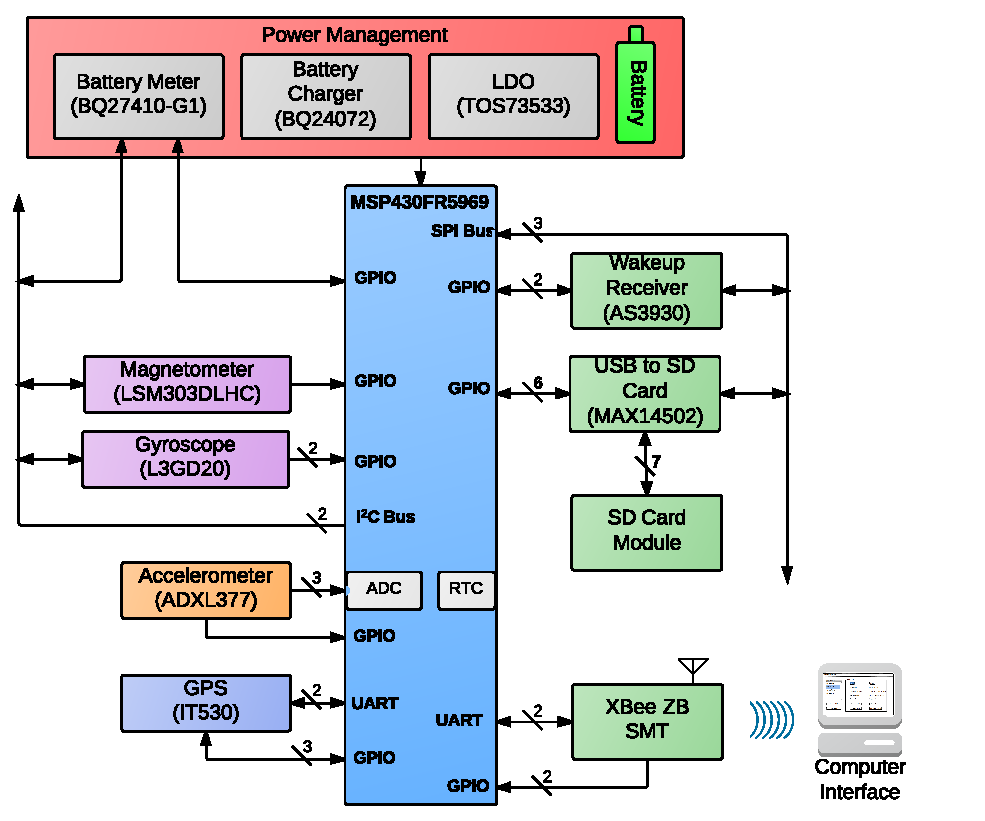
\includegraphics[width=0.95\textwidth]{img/blockDiagram}
	\caption{Block Diagram for the Drifter \label{fig:drifterBlockDiagram}}
\end{figure}

\subsection{Drifter Block Diagram}

\begin{enumerate}
\item \textbf{Microcontroller} -  Needed in order to be able to control and establish the communication between components as well as process the output of the sensors.

\item \textbf{Battery} - Required to provide the necessary power to the drifters because the electrical components are enclosed by a sphere.

\item \textbf{Power Management Circuit} - Composed of an LDO, a battery charger and a battery meter.  It is used to regulate the power provided by the battery, re-charge the battery once it has been depleted and to measure the amount of charge left on the battery.

\item \textbf{GPS Module} - Needed in order to know the precise location of the drifters when the user has to recover them after they have been thrown at sea for an experiment.

\item \textbf{Gyroscope} - Used to determine the rate of change of the orientation of the drifter while being carried by a wave.

\item \textbf{Accelerometer} - Used to measure the acceleration of the drifter while being carried by the waves.

\item \textbf{Magnetometer} - Used to determine the orientation of the drifter with respect to the Earth's magnetic north while it is being carried by a wave.

\item \textbf{Analog to Digital Converter (ADC)} - Needed in order to take the data from the accelerometer, which has an analog output, and convert it to digital signals so that the MCU can read them.  It is integrated within the MCU.

\item \textbf{SD Card and SD to USB Converter} - The SD Card is used to save the data captured by the sensors during an experiment.  The SD to USB converter will be used to allow the drifter to function as a mass storage device when connected to a Host computer via USB.

\item \textbf{XBee ZB Module} - Used to connect the spheres with a central base so that data can be retrieved without having to open the spheres.


\item \textbf{RF Wakeup Module} - Used to wirelessly wake up the drifter from low power mode via an RF signal.

\end{enumerate}

\begin{figure}[ht]
	\centering
	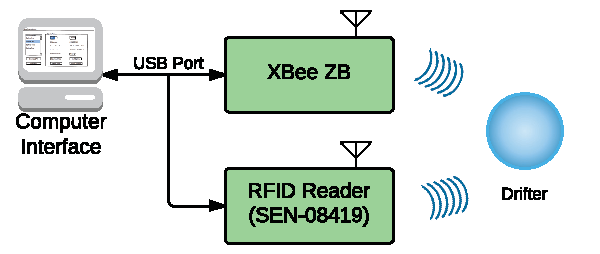
\includegraphics[scale=1]{img/baseBlockDiagram}
	\caption{Block Diagram for the Base Station \label{fig:baseBlockDiagram}}
\end{figure}

\subsection{Base Station Block Diagram}

\begin{enumerate}
\item \textbf{XBee ZB Module} -  Used to communicate with the drifters in order to send commands to switch operating modes and retrieve collected data.

\item \textbf{RFID Reader} - Used to generate the 125kHz signal required by the RF Wakeup module in the drifters to wake them up from low power mode.

\item \textbf{Computer} - Used to run a custom application that will be used to send commands and data to the drifters through the XBee.  A USB port in the computer will power the other devices in the base station.

\item \textbf{Power Management Circuit} - Composed of an LDO, a battery charger and a battery meter.  It is used to regulate the power provided by the battery, re-charge the battery once it has been depleted and to measure the amount of charge left on the battery.


\end{enumerate}
